% THIS DOCUMENT IS TAILORED TO REQUIREMENTS FOR SCIENTIFIC COMPUTING.  IT SHOULDN'T
% BE USED FOR NON-SCIENTIFIC COMPUTING PROJECTS
\documentclass[12pt]{article}

\usepackage{amsmath, mathtools}
\usepackage{amsfonts}
\usepackage{amssymb}
\usepackage{graphicx}
\usepackage{cite}
\usepackage{colortbl}
\usepackage{xr}
\usepackage{hyperref}
\usepackage{longtable}
\usepackage{xfrac}
\usepackage{tabularx}
\usepackage{float}
\usepackage{siunitx}
\usepackage{booktabs}
\usepackage{caption}
\usepackage{pdflscape}
\usepackage{afterpage}
\usepackage{datetime2}

\usepackage[round]{natbib}

%\usepackage{refcheck}

\hypersetup{
    bookmarks=true,         % show bookmarks bar?
      colorlinks=true,       % false: boxed links; true: colored links
    linkcolor=red,          % color of internal links (change box color with linkbordercolor)
    citecolor=green,        % color of links to bibliography
    filecolor=magenta,      % color of file links
    urlcolor=cyan           % color of external links
}

%% Comments

\usepackage{color}

\newif\ifcomments\commentstrue %displays comments
%\newif\ifcomments\commentsfalse %so that comments do not display

\ifcomments
\newcommand{\authornote}[3]{\textcolor{#1}{[#3 ---#2]}}
\newcommand{\todo}[1]{\textcolor{red}{[TODO: #1]}}
\else
\newcommand{\authornote}[3]{}
\newcommand{\todo}[1]{}
\fi

\newcommand{\wss}[1]{\authornote{blue}{SS}{#1}} 
\newcommand{\plt}[1]{\authornote{magenta}{TPLT}{#1}} %For explanation of the template
\newcommand{\an}[1]{\authornote{cyan}{Author}{#1}}

%% Common Parts

\newcommand{\progname}{ProgName} % PUT YOUR PROGRAM NAME HERE
\newcommand{\authname}{Team \#, Team Name
\\ Student 1 name
\\ Student 2 name
\\ Student 3 name
\\ Student 4 name} % AUTHOR NAMES                  

\usepackage{hyperref}
    \hypersetup{colorlinks=true, linkcolor=blue, citecolor=blue, filecolor=blue,
                urlcolor=blue, unicode=false}
    \urlstyle{same}
                                


% For easy change of table widths
\newcommand{\colZwidth}{1.0\textwidth}
\newcommand{\colAwidth}{0.13\textwidth}
\newcommand{\colBwidth}{0.82\textwidth}
\newcommand{\colCwidth}{0.1\textwidth}
\newcommand{\colDwidth}{0.05\textwidth}
\newcommand{\colEwidth}{0.8\textwidth}
\newcommand{\colFwidth}{0.17\textwidth}
\newcommand{\colGwidth}{0.5\textwidth}
\newcommand{\colHwidth}{0.28\textwidth}

% Used so that cross-references have a meaningful prefix
\newcounter{defnum} %Definition Number
\newcommand{\dthedefnum}{GD\thedefnum}
\newcommand{\dref}[1]{GD\ref{#1}}
\newcounter{datadefnum} %Datadefinition Number
\newcommand{\ddthedatadefnum}{DD\thedatadefnum}
\newcommand{\ddref}[1]{DD\ref{#1}}
\newcounter{theorynum} %Theory Number
\newcommand{\tthetheorynum}{TM\thetheorynum}
\newcommand{\tref}[1]{TM\ref{#1}}
\newcounter{tablenum} %Table Number
\newcommand{\tbthetablenum}{TB\thetablenum}
\newcommand{\tbref}[1]{TB\ref{#1}}
\newcounter{assumpnum} %Assumption Number
\newcommand{\atheassumpnum}{A\theassumpnum}
\newcommand{\aref}[1]{A\ref{#1}}
\newcounter{goalnum} %Goal Number
\newcommand{\gthegoalnum}{GS\thegoalnum}
\newcommand{\gsref}[1]{GS\ref{#1}}
\newcounter{instnum} %Instance Number
\newcommand{\itheinstnum}{IM\theinstnum}
\newcommand{\iref}[1]{IM\ref{#1}}
\newcounter{reqnum} %Requirement Number
\newcommand{\rthereqnum}{R\thereqnum}
\newcommand{\rref}[1]{R\ref{#1}}
\newcounter{nfrnum} %NFR Number
\newcommand{\rthenfrnum}{NFR\thenfrnum}
\newcommand{\nfrref}[1]{NFR\ref{#1}}
\newcounter{lcnum} %Likely change number
\newcommand{\lthelcnum}{LC\thelcnum}
\newcommand{\lcref}[1]{LC\ref{#1}}

\usepackage{fullpage}
\newcounter{theornum} %Theory Number
\newcommand{\deftheory}[9][Not Applicable]
{
\newpage
\noindent \rule{\textwidth}{0.5mm}

\paragraph{RefName: } \textbf{#2} \phantomsection 
\label{#2}

\paragraph{Label:} #3

\noindent \rule{\textwidth}{0.5mm}

\paragraph{Equation:}

#4

\paragraph{Description:}

#5

\paragraph{Notes:}

#6

\paragraph{Source:}

#7

\paragraph{Ref.\ By:}

#8

\paragraph{Preconditions for \hyperref[#2]{#2}:}
\label{#2_precond}

#9

\paragraph{Derivation for \hyperref[#2]{#2}:}
\label{#2_deriv}

#1

\noindent \rule{\textwidth}{0.5mm}

}

\begin{document}

\title{Software Requirements Specification for \progname: subtitle describing software} 
\author{\authname}
\date{\today}
	
\maketitle

~\newpage

\pagenumbering{roman}

\tableofcontents

~\newpage

\section*{Revision History}

\begin{tabularx}{\textwidth}{p{3cm}p{2cm}X}
\toprule {\bf Date} & {\bf Version} & {\bf Notes}\\
\midrule
2022-02-05 & 1.0 & Initial Release\\
\bottomrule
\end{tabularx}
~\newpage

\section{Reference Material}

This section records information for easy reference.

\subsection{Table of Units}

Throughout this document SI (Syst\`{e}me International d'Unit\'{e}s) is employed
as the unit system.  In addition to the basic units, several derived units are
used as described below.  For each unit, the symbol is given followed by a
description of the unit and the SI name.
~\newline

\renewcommand{\arraystretch}{1.2}
%\begin{table}[ht]
  \noindent \begin{tabular}{l l l} 
    \toprule		
    \textbf{symbol} & \textbf{unit} & \textbf{SI}\\
    \midrule 
    \si{\metre} & length & metre\\
    \si{\second} & time & second\\
    \bottomrule
  \end{tabular}
  %	\caption{Provide a caption}
%\end{table}

\plt{Only include the units that your SRS actually uses.}

\plt{Derived units, like newtons, pascal, etc, should show their derivation
    (the units they are derived from) if their constituent units are in the
    table of units (that is, if the units they are derived from are used in the
    document).  For instance, the derivation of pascals as
    $\si{\pascal}=\si{\newton\per\square\meter}$ is shown if newtons and m are
    both in the table.  The derivations of newtons would not be shown if kg and
    s are not both in the table.}

\plt{The symbol for units named after people use capital letters, but the name
  of the unit itself uses lower case.  For instance, pascals use the symbol Pa,
  watts use the symbol W, teslas use the symbol T, newtons use the symbol N,
  etc.  The one exception to this is degree Celsius.  Details on writing metric
  units can be found on the 
  \href{https://www.nist.gov/pml/weights-and-measures/writing-metric-units}
  {NIST} web-page.}

\subsection{Table of Symbols}

The table that follows summarizes the symbols used in this document along with
their units.  The choice of symbols was made to be consistent with the heat
transfer literature and with existing documentation for solar water heating
systems.  The symbols are listed in alphabetical order.

\renewcommand{\arraystretch}{1.2}
%\noindent \begin{tabularx}{1.0\textwidth}{l l X}
\noindent \begin{longtable*}{l l p{12cm}} \toprule
\textbf{symbol} & \textbf{unit} & \textbf{description}\\
\midrule 
$i$ & Unitless & Robot pose instance
\\
$j$ &	Unitless & Camera Instance
\\
$k$ &	Unitless & Target Feature Instance
\\
$\textbf{A}$ & 3$\times$4 Matrix & SE(3) Equivalent transformation of a camera 
with respect to the target feature frame
\\
$\textbf{B}$ & 3$\times$4 Matrix & SE(3) Equivalent transformation of the 
end-effector in the robot-base frame
\\
$\textbf{R}$ & 3$\times$3 Matrix & Rotation matrix in SO(3)
\\
$\textit{t}$ & 3$\times$3 Matrix & Translation matrix in SE(3)
\\
$\textbf{X}$ & 3$\times$4 Matrix & SE(3) Equivalent transformation of the target 
feature in the robot-base frame
\\
$\textbf{Y}$ & 3$\times$4 Matrix & SE(3) Equivalent transformation of the camera 
in the end-effector frame
\\ 
\bottomrule
\end{longtable*}
\plt{Use your problems actual symbols.  The si package is a good idea to use for
  units.}

\subsection{Abbreviations and Acronyms}

\renewcommand{\arraystretch}{1.2}
\begin{tabular}{l l} 
  \toprule		
  \textbf{symbol} & \textbf{description}\\
  \midrule 
  A & Assumption\\
  BRIEF & Binary Robust Independent Elementary Features\\ 
  DD & Data Definition\\
  IFC & \progname{}\\
  FAST & Features from Accelerated Segment Test\\
  FOV & Field-of-View\\
  GD & General Definition\\
  GS & Goal Statement\\
  HERW  & Hand-Eye Robot-World Formulation \\
  IM & Instance Model\\
  LC & Likely Change\\
  ORB & Oriented FAST and Rotated BRIEF\\
  PS & Physical System Description\\
  R & Requirement\\
  SRS & Software Requirements Specification\\
  SURF & Speeded-Up Robust Features\\
  TM & Theoretical Model\\
  V\&V & Verification and Validation\\
  \bottomrule
\end{tabular}\\

\plt{Add any other abbreviations or acronyms that you add}

\subsection{Mathematical Notation}

\begin{itemize}
  \item Matrixes are capitalized and are bolded, i.e. $\mathbf{X, Y}$
  \item Column vectors are lowercase and are bolded, i.e. $\mathbf{s, t}$
  \item Scalars are lowercase and are not bolded, i.e.\ a, b
\end{itemize}

\plt{This section is optional, but should be included for projects that make use
  of notation to convey mathematical information.  For instance, if typographic
  conventions (like bold face font) are used to distinguish matrices, this
  should be stated here.  If symbols are used to show mathematical operations,
  these should be summarized here.  In some cases the easiest way to summarize
  the notation is to point to a text or other source that explains the
  notation.}

\plt{This section was added to the template because some students use very
  domain specific notation.  This notation will not be readily understandable to
  people outside of your domain.  It should be explained.}

\newpage

\pagenumbering{arabic}

\plt{Guiding principles for the SRS document:
\begin{itemize}
\item Do not repeat the same information at the same abstraction level.  If
  information is repeated, the repetition should be at a different abstraction
  level.  For instance, there will be overlap between the scope section and the
  assumptions, but the scope section will not go into as much detail as the
  assumptions section.
\end{itemize}
}

\plt{When the documentation is done, it should be possible to trace back to the
  source of every piece of information.  Some information will come from
  external sources, like terminology.  Other information will be derived, like
  General Definitions.}

\plt{An SRS document should have the following qualities: unambiguous,
  consistent, complete, validatable, abstract and traceable.}

\plt{The overall goal of the SRS is that someone that meets the Characteristics
  of the Intended Reader (Section~\ref{sec_IntendedReader}) can learn,
  understand and verify the captured domain knowledge.  They should not have to
  trust the authors of the SRS on any statements.  They should be able to
  independently verify/derive every statement made.}

\section{Introduction}
Camera sensors are a common choice of sensor for many applications in robotics due 
in part to their low cost and ease of integration. Prior to their use, each camera 
must be calibrated such that collected data in collected imagery can be aligned with 
the 3D world. This process is essential to prepare the system so that 
imagery data can be correctly captured and processed for downstream operations.

Camera calibration consists of two aspects; intrinsic calibration and extrinsic 
calibration. Intrinsic calibration focuses on mapping the 2D camera image 
to the 3D camera frame, Extrinsic calibration converts the 3D camera frame
to a global world frame. Extrinsic calibration is of significant interest as  
operators may need to reposition cameras on a robotic platforms for any number of 
operational needs.

The following section outlines the Software Requirements Specification (SRS) for 
a calibration algorithm that calculates the extrinsic parameters for a multi-camera 
robotic platform. The program may be refered to as Image Feature Correspondences, 
or IFC.



\subsection{Purpose of Document}

This document is the primary resource for the user to outline the desired 
characteristics of the user, the required system interfaces, and desired 
integrated behaviour of the IFC algorithm. The goals and key assumptions of the
desired software are outlined, in addition to the required definitions, 
theoretical models and instance models required to support its development. 
Specifically, theoretical models are outlined to provide a framework to promote 
development such that a specific design solution is not imposed at an early stage 
of development. The SRS is abstract - it bounds what problems need to be solved by 
the system, rather than how it needs to be achieved.

Following a standard waterfall development model, this document will be used as a 
stepping to support the development of several additional documents, each of which 
demonstrates successive growth in the understanding and maturation of the software 
product. These documents include:
\begin{enumerate}
  \item The Design Specification: An outline of the architectural decisions that 
  details   how the requirements will be realized in the system. This is inclusive 
  of the choice of operating environment, system interfaces with the user and its 
  environment, and the   numerical methods that shall be implemented.

  \item The Verification and Validation (V\&V) Plan: An outline of the specific processess 
  to be used to assess the implementation of the code as developed from the Design 
  Specification. Verification assessments will be used to assess whether the system has been 
  built to the specified requirements from the SRS. Validation tests may also be outlined to 
  ensure that the software correctly addresses the problem as defined in  build confidence 
  that the   design has satisfied the outlined requirements per \ref{Sec_pd}.
\end{enumerate}


\subsection{Scope of Requirements} 
The outlined requirements includes conventional imagery processing algorithms. When supplied 
with the permissible inputs, the IFC software shall is intended to scan imagery data to and 
identify match candidates amongst each image for various cameras and robot pose.The entire 
document is written under the assumption that that the within the imagery scene 
is free of significant changes in ambient illumination during imagery capture. Camera 
intrinsics are expected to be prior to compile time.



\plt{Modelling the real world requires simplification.  The full complexity of
  the actual physics, chemistry, biology is too much for existing models, and
  for existing computational solution techniques.  Rather than say what is in
  the scope, it is usually easier to say what is not.  You can think of it as
  the scope is initially everything, and then it is constrained to create the
  actual scope.  For instance, the problem can be restricted to 2 dimensions, or
  it can ignore the effect of temperature (or pressure) on the material
  properties, etc.}  
 
\plt{The scope section is related to the assumptions section
  (Section~\ref{sec_assumpt}).  However, the scope and the assumptions are not
  at the same level of abstraction.  The scope is at a high level.  The focus is
  on the ``big picture'' assumptions.  The assumptions section lists, and
  describes, all of the assumptions.}

\plt{The scope section is relevant for later determining typical values of inputs. 
The scope should make it clear what inputs are reasonable to expect. This is a 
distinction between scope and context (context is a later section).  Scope affects 
the inputs while context affects how the software will be used.}

\subsection{Characteristics of Intended Reader} \label{sec_IntendedReader}
Reviewers of this document should have a , 
and a strong understanding of image processing algorithms. A 4th year undergraduate or 
Master's level course in Computer Vision algorithm is strongly recommended. The 
reviewer should have an understanding of robot mechanics per a 3rd or 4th year 
undergraduate course. The developer should also have a general background in statistics 
and functional programming.


\plt{This section summarizes the skills and knowledge of the readers of the
  SRS.  It does NOT have the same purpose as the ``User Characteristics''
  section (Section~\ref{SecUserCharacteristics}).  The intended readers are the
  people that will read, review and maintain the SRS.  They are the people that
  will conceivably design the software that is intended to meet the
  requirements.  The user, on the other hand, is the person that uses the
  software that is built.  They may never read this SRS document.  Of course,
  the same person could be a ``user'' and an ``intended reader.''}

\plt{The intended reader characteristics should be written as unambiguously and
  as specifically as possible.  Rather than say, the user should have an
  understanding of physics, say what kind of physics and at what level.  For
  instance, is high school physics adequate, or should the reader have had a
  graduate course on advanced quantum mechanics?}

\subsection{Organization of Document}
The remainder of the document uses a top-down structure that outlines, in order, 
the goals, assumptions, theories, definitions, and instance models. These 
components are then used to derive the functional and non-functional requirements. 
Goal statements and assumptions are sequentially distilled into theoretical models, 
definitions, instance models, and finally to requirements.

The reader can glean value through review of the instance models prior to 
the theoretical models, as the instance models outlne an operational specification of 
system behaviour, rather than a descriptive specification. This enables flexibility 
in what theoretical models are applied as they may be selected as inputs to the 
systems as a functional program. 

\plt{This section provides a roadmap of the SRS document.  It will help the
  reader orient themselves.  It will provide direction that will help them
  select which sections they want to read, and in what order.  This section will
  be similar between project.}

\section{General System Description}

This section provides general information about the system.  It identifies the
interfaces between the system and its environment, describes the user
characteristics and lists the system constraints.

\plt{The purpose of this section is to provide general information about the
  system so the specific requirements in the next section will be easier to
  understand. The general system description section is designed to be
  changeable independent of changes to the functional requirements documented in
  the specific system description. The general system description provides a
  context for a family of related models.  The general description can stay the
  same, while specific details are changed between family members.}

\subsection{System Context}
Figure \ref{Fig_SystemContext} depicts the system context. A rectangle represents 
the IFC software itself, whereas circles depict interactions with stakeholders, 
namely the user. Arrowheads are used to demonstrate the sequential flow of data 
between the software system and the environment.

\begin{figure}[h!]
\begin{center}
 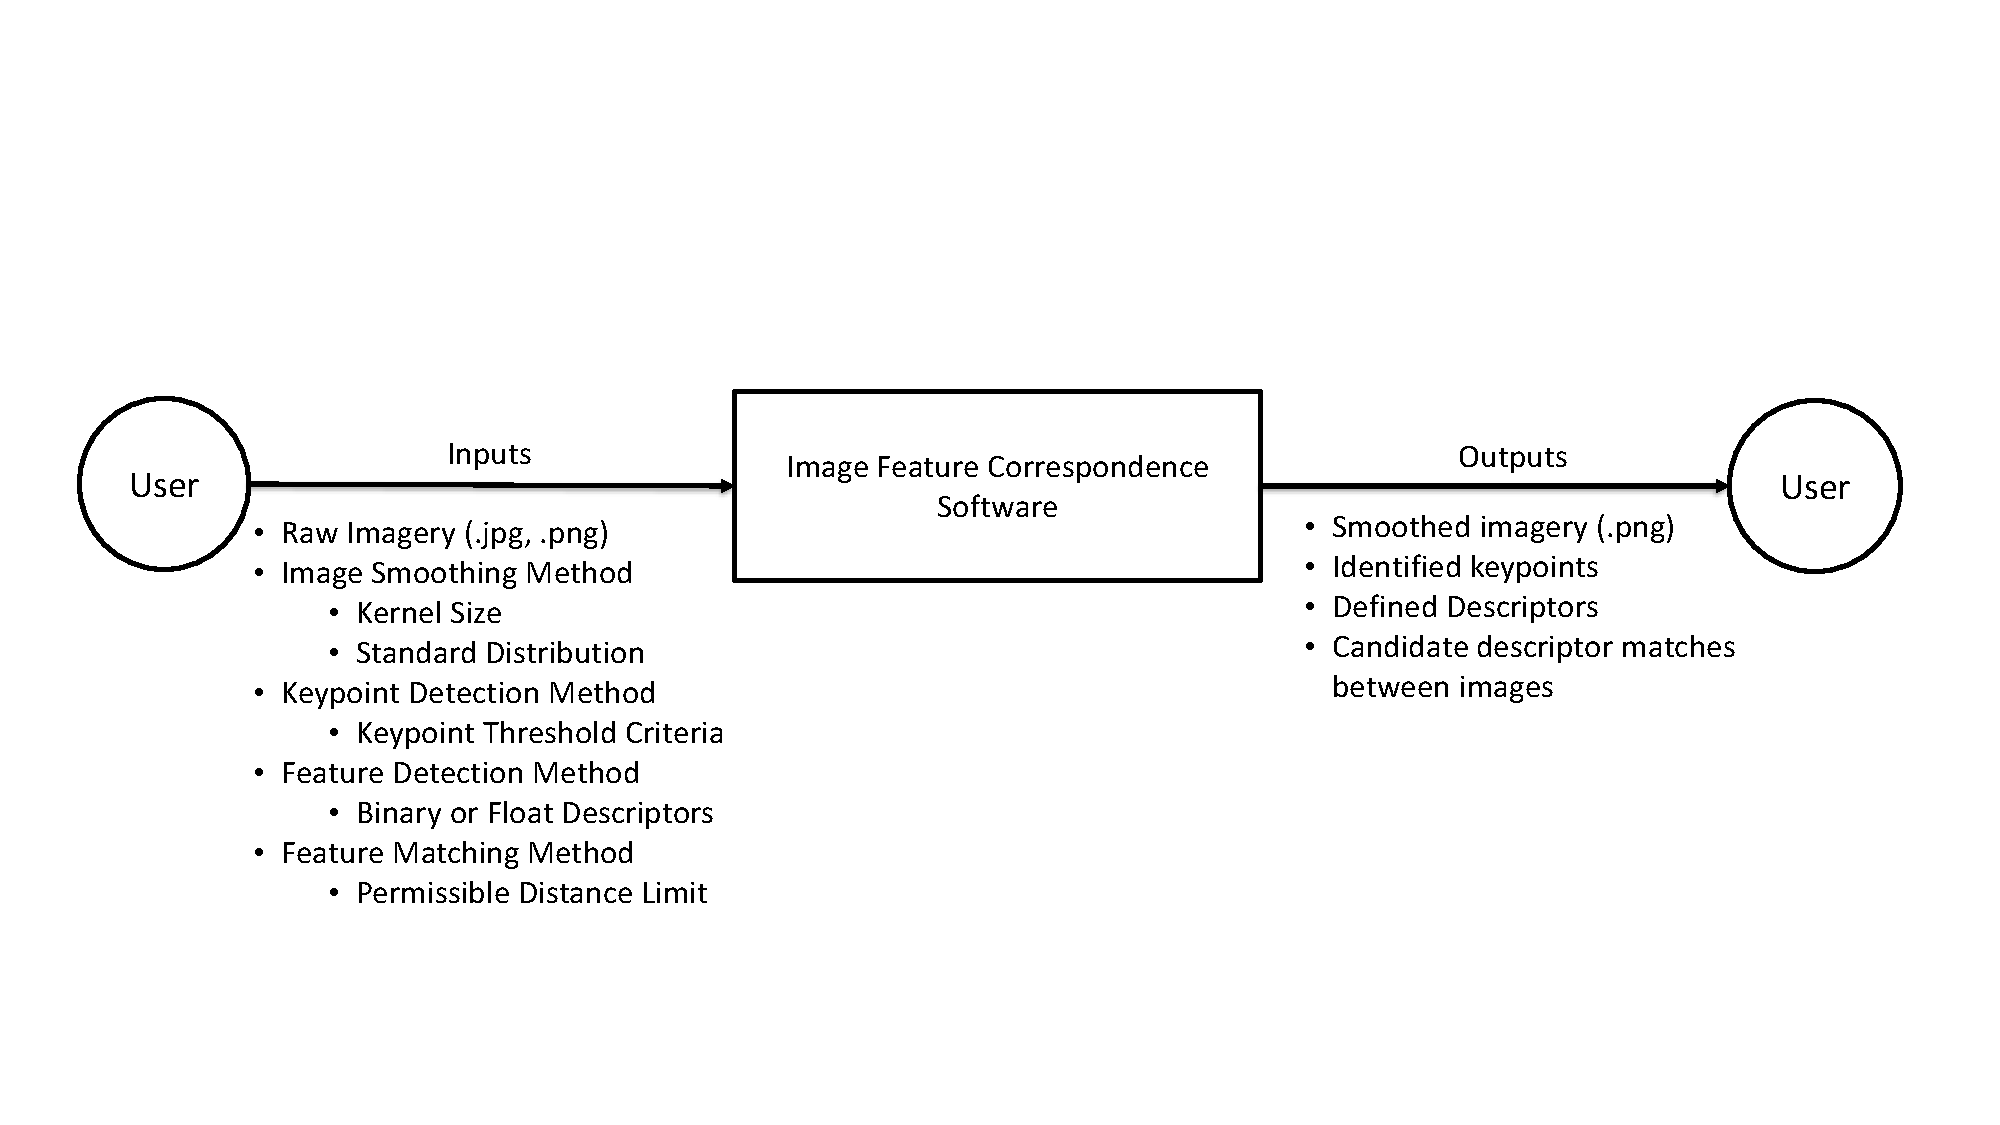
\includegraphics[width=0.6\textwidth]{SystemContextFigure}
\caption{System Context}
\label{Fig_SystemContext} 
\end{center}
\end{figure}

\plt{For each of the entities in the system context diagram its responsibilities
  should be listed.  Whenever possible the system should check for data quality,
  but for some cases the user will need to assume that responsibility.  The list
  of responsibilities should be about the inputs and outputs only, and they
  should be abstract.  Details should not be presented here.  However, the
  information should not be so abstract as to just say ``inputs'' and
  ``outputs''.  A summarizing phrase can be used to characterize the inputs.
  For instance, saying ``material properties'' provides some information, but it
  stays away from the detail of listing every required properties.}

\begin{itemize}
\item User Responsibilities:
\begin{itemize}
\item Provide input data to the system
\item Verify that the input data uses the correct units
\item Verify that the input data is contained in the correct data structures
\item Configure the type of feature-handler algorithms to be used with corresponding 
threshold criteria
\end{itemize}
\item \progname{} Responsibilities:
\begin{itemize}
\item Detect data type mismatch, such as a string of characters instead of a
  floating point number
\item Assess whether inputs constitute a fully define physical setup
\item Calculate required outputs
\end{itemize}
\end{itemize}

\plt{Identify in what context the software will typically be used.  Is it for
exploration? education? engineering work? scientific work?. Identify whether it
will be used for mission-critical or safety-critical applications.} \plt{This
additional context information is needed to determine how much effort should be
devoted to the rationale section.  If the application is safety-critical, the
bar is higher.  This is currently less structured, but analogous to, the idea to
the Automotive Safety Integrity Levels (ASILs) that McSCert uses in their
automotive hazard analyses.}

\subsection{User Characteristics} \label{SecUserCharacteristics}
The end user of the IFC software should have an undergraduate understanding of introductory 
mechanicas of robots, statistics, and computer vision algorithms.

\plt{This section summarizes the knowledge/skills expected of the user.
  Measuring usability, which is often a required non-function requirement,
  requires knowledge of a typical user.  As mentioned above, the user is a
  different role from the ``intended reader,'' as given in
  Section~\ref{sec_IntendedReader}.  As in Section~\ref{sec_IntendedReader}, the
  user characteristics should be specific an unambiguous.  For instance, ``The
  end user of \progname{} should have an understanding of undergraduate Level 1
  Calculus and Physics.''}

\subsection{System Constraints}

\plt{System constraints differ from other type of requirements because they
  limit the developers' options in the system design and they identify how the
  eventual system must fit into the world. This is the only place in the SRS
  where design decisions can be specified.  That is, the quality requirement for
  abstraction is relaxed here.  However, system constraints should only be
  included if they are truly required.}

\section{Specific System Description}
This section first presents the problem description, which gives a high-level
view of the problem to be solved.  This is followed by the solution characteristics
specification, which presents the assumptions, theories, definitions and finally
the instance models. 

\subsection{Problem Description} \label{Sec_pd}

\progname{} is intended to evaluate how imagery data from robot-based cameras can 
can be manipulated to define and align features between separate images in support 
of downstream operations for extrinsic camera calibration.

\subsubsection{Terminology and  Definitions}

This subsection provides a list of terms that are used in the subsequent
sections and their meaning, with the purpose of reducing ambiguity and making it
easier to correctly understand the requirements:

\begin{itemize}

\item Features: Distinctive patterns or structures in an image that are 
identifiable and useful for matching between images

\item Keypoints: Specific pixel locations in an image that represent 
significant and repeatable features.

\item Correspondences: Pairs of keypoints between two images that represent 
represent the same real-world point.

\item Extrinsic Parameters: The transform of the between the 3D camera frame to the 
3D world frame.

\item Intrinsic Parameters: camera parameters that pertain to the transform of the 
2D image plane frame to the 3D camera frame.

\item Hand-eye: the relation between the robot end-effector to the camera frame

\item Robot-world: the relation between the robot base frame to the world frame

\item Pose: refers to the position and orientation of an object, sensor, or robot 
within a given reference frame. 

\item Patch: A square region of an image of an assigned size.
\end{itemize}

\subsubsection{Physical System Description} \label{sec_phySystDescrip}
The physical system of \progname{}, as shown in Figure \ref{Wang_EOH}, outlines 
case of a single-camera, single target configuration. This outlines the frames of 
interest for \ref{PS_1}. This configuration can be extrapolated to the multi-camera, 
multi-target case, as shown in \ref{PS_2}. A representation of equivalent keypoints 
between images is shown in \ref{PS_3}.
\\
\\
\noindent \label{PS_1}PS1: Frames for the robot base, hand, camera, and target landmark
\noindent \label{PS_2}PS2: Known base-to-hand transform.
\noindent \label{PS_3}PS3: Projected camera images from distinct camera poses.

\plt{The purpose of this section is to clearly and unambiguously state the
  physical system that is to be modelled. Effective problem solving requires a
  logical and organized approach. The statements on the physical system to be
  studied should cover enough information to solve the problem. The physical
  description involves element identification, where elements are defined as
  independent and separable items of the physical system. Some example elements
  include acceleration due to gravity, the mass of an object, and the size and
  shape of an object. Each element should be identified and labelled, with their
  interesting properties specified clearly. The physical description can also
  include interactions of the elements, such as the following: i) the
  interactions between the elements and their physical environment; ii) the
  interactions between elements; and, iii) the initial or boundary conditions.}

\plt{The elements of the physical system do not have to correspond to an actual
physical entity.  They can be conceptual.  This is particularly important when
the documentation is for a numerical method.}


\begin{figure}[h!]
  \begin{center}
  \centering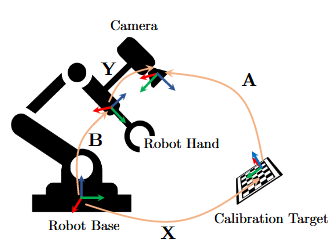
\includegraphics[width=0.5\textwidth]{Images/Wang_EOH.png}
  \caption{Single-camera robotic manipulator robot-world hand eye 
  configuration. Modified from \cite{Wang_2022}.}.
  \label{Wang_EOH}
  \end{center}
\end{figure}

\begin{figure}[ht!]
  \begin{center}
  \centering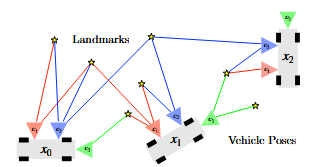
\includegraphics[width=0.5\textwidth]{Images/OASIS_CFG.png}
  \caption{Multi-camera mobile robotic platform. 
  Modified from \cite{OASIS_2024}.}.
  \label{OASIS}
  \end{center}
\end{figure}

\begin{figure}[ht!]
  \begin{center}
  \centering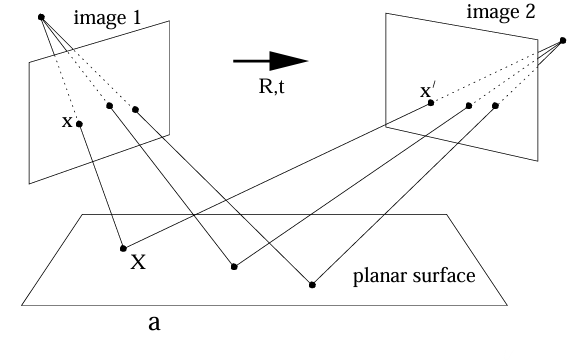
\includegraphics[width=0.5\textwidth]{Images/MULTIVIEW.png}
  \caption{Multi-camera mobile robotic platform. 
  Modified from \cite{Hartley_Zisserman}.}.
  \label{MV_HZ}
  \end{center}
\end{figure}






\subsubsection{Goal Statements}

\plt{The goal statements refine the ``Problem Description''
  (Section~\ref{Sec_pd}).  A goal is a functional objective the system under
  consideration should achieve. Goals provide criteria for sufficient
  completeness of a requirements specification and for requirements
  pertinence. Goals will be refined in Section “Instanced Models”
  (Section~\ref{sec_instance}). Large and complex goals should be decomposed
  into smaller sub-goals.  The goals are written abstractly, with a minimal
  amount of technical language.  They should be understandable by non-domain
  experts.}

\noindent Given the \plt{inputs}, the goal statements are:

\begin{itemize}

  \item[GS\refstepcounter{goalnum}\thegoalnum \label{define_features}:]
    Define the method(s) used to search for feature correspondences between each image frame.
    
  \item[GS\refstepcounter{goalnum}\thegoalnum \label{compare_features}:]
    Define the method(s) used to search for feature correspondences between each image frame.
  
  \item[GS\refstepcounter{goalnum}\thegoalnum \label{identify_features}:]
    Identify a collection of features from each image frame. 
  
  \item[GS\refstepcounter{goalnum}\thegoalnum \label{identify_matches}:] 
    Identify feature correspondences between images.
  
  \item[GS\refstepcounter{goalnum}\thegoalnum \label{report_matches}:]
    Generate a report of the identified feature correspondences.
    
\end{itemize}

\subsection{Solution Characteristics Specification}

\plt{This section specifies the information in the solution domain of the system
  to be developed. This section is intended to express what is required in
  such a way that analysts and stakeholders get a clear picture, and the
  latter will accept it. The purpose of this section is to reduce the problem
  into one expressed in mathematical terms. Mathematical expertise is used to
  extract the essentials from the underlying physical description of the
  problem, and to collect and substantiate all physical data pertinent to the
  problem.}

\plt{This section presents the solution characteristics by successively refining
  models.  It starts with the abstract/general Theoretical Models (TMs) and
  refines them to the concrete/specific Instance Models (IMs).  If necessary
  there are intermediate refinements to General Definitions (GDs).  All of these
  refinements can potentially use Assumptions (A) and Data Definitions (DD).
  TMs are refined to create new models, that are called GMs or IMs. DDs are not
  refined; they are just used. GDs and IMs are derived, or refined, from other
  models. DDs are not derived; they are just given. TMs are also just given, but
  they are refined, not used.  If a potential DD includes a derivation, then
  that means it is refining other models, which would make it a GD or an IM.}

\plt{The above makes a distinction between ``refined'' and ``used.'' A model is
  refined to another model if it is changed by the refinement. When we change a
  general 3D equation to a 2D equation, we are making a refinement, by applying
  the assumption that the third dimension does not matter. If we use a
  definition, like the definition of density, we aren't refining, or changing
  that definition, we are just using it.}

\plt{The same information can be a TM in one problem and a DD in another.  It is
  about how the information is used.  In one problem the definition of
  acceleration can be a TM, in another it would be a DD.}

\plt{There is repetition between the information given in the different chunks
  (TM, GDs etc) with other information in the document.  For instance, the
  meaning of the symbols, the units etc are repeated.  This is so that the
  chunks can stand on their own when being read by a reviewer/user.  It also
  facilitates reuse of the models in a different context.}

\noindent \plt{The relationships between the parts of the document are show in
  the following figure.  In this diagram ``may ref'' has the same role as
  ``uses'' above.  The figure adds ``Likely Changes,'' which are able to
  reference (use) Assumptions.}

\begin{figure}[H]
  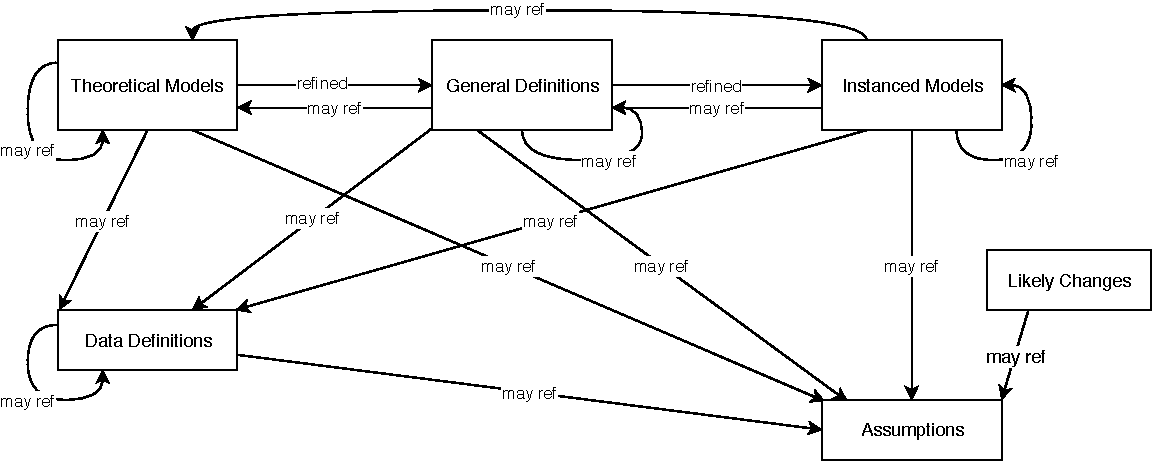
\includegraphics[scale=0.9]{RelationsBetweenTM_GD_IM_DD_A.pdf}
\end{figure}

The instance models that govern \progname{} are presented in
Subsection~\ref{sec_instance}.  The information to understand the meaning of the
instance models and their derivation is also presented, so that the instance
models can be verified.

\subsubsection{Types}

\plt{This section is optional. Defining types can make the document easier to
understand.}

\subsubsection{Scope Decisions}
Control of the ambient illumination conditions falls outside the scope of this software.
It is the responsibility of the user to verify that the ambient lighting conditions do 
not change to a significant degree during the image capture process.


\subsubsection{Modelling Decisions}

\plt{This section is optional.}

\subsubsection{Assumptions} \label{sec_assumpt}
\plt{If it helps with the organization and understandability, the assumptions
can be presented as sub sections.  The following sub-sections are options:
background theory assumptions, helper theory assumptions, generic theory
assumptions, problem specific assumptions, and rationale assumptions}

This section simplifies the original problem and helps in developing the
theoretical model by filling in the missing information for the physical system.
The numbers given in the square brackets refer to the theoretical model [TM],
general definition [GD], data definition [DD], instance model [IM], or likely
change [LC], in which the respective assumption is used.

\begin{itemize}
\item[A\refstepcounter{assumpnum}\theassumpnum \label{A:min_num_cameras}:]
Imagery shall be provided by at least one camera \dref{TM_Dist_Ham}.

\item[A\refstepcounter{assumpnum}\theassumpnum \label{A:camera_model}:]
All supplied imagery is produced by a pinhole model, affine camera 
\dref{GD_2D_Gauss}, \dref{GD_FAST}, \dref{GD_rBRIEF}.

\item[A\refstepcounter{assumpnum}\theassumpnum \label{A:greyscale}:]
All imagery will be input as greyscale data \dref{GD_2D_Gauss}.

\item[A\refstepcounter{assumpnum}\theassumpnum \label{A:RT_Memory}:]
The solution is not limited to memory constraints observed in hardware used for real-time 
applications (\tref{TM_BRIEF}).

\end{itemize}

\subsubsection{Theoretical Models}\label{sec_theoretical}

\plt{Theoretical models are sets of abstract mathematical equations or axioms
  for solving the problem described in Section ``Physical System Description''
  (Section~\ref{sec_phySystDescrip}). Examples of theoretical models are
  physical laws, constitutive equations, relevant conversion factors, etc.}

\plt{Optionally the theory section could be divided into subsections to provide
more structure and improve understandability and reusability.  Potential
subsections include the following: Context theories, background theories, helper
theories, generic theories, problem specific theories, final theories and
rationale theories.}

This section focuses on the general equations and laws that \progname{} is based
on.  \plt{Modify the examples below for your problem, and add additional models
  as appropriate.}

~\newline



% Theoretical Model 1
\noindent
\begin{minipage}{\textwidth}
\renewcommand*{\arraystretch}{1.5}
\begin{tabular}{| p{\colAwidth} | p{\colBwidth}|}
\hline
\rowcolor[gray]{0.9}
Number& TM\refstepcounter{theorynum}\thetheorynum \label{TM_ND_Gauss}\\
\hline
Label &\bf N-Dimensional Gaussian Kernel \\
\hline
Equation&$G_{N-Dim}(\overrightarrow{x},\sigma) = \frac{1}{2\pi\sigma^2}e^{-\frac{\overrightarrow{x}}
{2\sigma^2}}$  \\
\hline
Description & The above equation represents the distribution of data when defined as a n-dimensional  
Gaussian Distribution. $\overrightarrow{x}$ is the collection of n-dimensions in the 
Gaussian distribution. $\sigma$ is the standard deviation of the Gaussian distribution. 
\\
\hline
Notes & All variables are unitless. \\
\hline
Source & \cite{Gauss_Kernel} \\
\hline
Ref.\ By & \dref{GD_2D_Gauss}\\
\hline
Pre-conditions for TM\thetheorynum: &None \\
\hline
Derivation for TM\thetheorynum: &None \\
\hline
\end{tabular}
\end{minipage}\\



% Theoretical Model 2
\noindent
\begin{minipage}{\textwidth}
\renewcommand*{\arraystretch}{1.5}
\begin{tabular}{| p{\colAwidth} | p{\colBwidth}|}
\hline
\rowcolor[gray]{0.9}
Number& TM\refstepcounter{theorynum}\thetheorynum \label{TM_FAST}\\
\hline
Label &\bf Features from Accelerated Segment Test (FAST)  \\
\hline
Equation& $S_{p \rightarrow x} = \begin{cases} 
  \mathit{d, , I_{p \rightarrow x} \leq I_{p} - t} \quad\textnormal{(darker)} \\
  \mathit{s, , I_{p \rightarrow x} \leq I_{p} + t} \quad\textnormal{(similar)} \\
  \mathit{b, , I_{p} + t \leq I_{p \rightarrow x} \quad\textnormal{(brighter)}} \\
  \end{cases}
$  \\
\hline
Description & $\mathit{x}$ represents the 16 contiguous pixels that surround pixel $\mathit{p}$, or 
$\mathit{x} \in \{1,...,16\}$. 
$S_{p \rightarrow x}$ represents the comparison of pixel intensity for $\mathit{p}$ to $\mathit{x}$, 
with an assignment of $\mathit{d, s}$, or $\mathit{b}$ to represent that pixel $\mathit{p}$ is brighter, 
darker, or similar to its neighbours. If the pixel is classified as either a $\mathit{b}$ or a 
$\mathit{d}$, then the pixel is defined as a keypoint for edge detection.
\\
\hline
Notes & All variables are unitless. \\
\hline
Source & \cite{FAST} \\
\hline
Ref.\ By & \dref{GD_FAST}, \lcref{keypoint_method}\\
\hline
Pre-conditions for TM\thetheorynum: &None \\
\hline
Derivation for TM\thetheorynum: &None \\
\hline
\end{tabular}
\end{minipage}\\



% Theoretical Model 3
\noindent
\begin{minipage}{\textwidth}
\renewcommand*{\arraystretch}{1.5}
\begin{tabular}{| p{\colAwidth} | p{\colBwidth}|}
\hline
\rowcolor[gray]{0.9}
Number& TM\refstepcounter{theorynum}\thetheorynum \label{TM_BRIEF}\\
\hline
Label &\bf Binary Robust Independent Elementary Features (BRIEF)  \\
\hline
Equation& $\mathit{d_{k}}= \mathbf{1}({\mathit{I(p_{k})< I(q_{k})}})$
\\
\hline
Description & For a selected patch within an image, and $\mathit{d_{k}}$ represents the kth bit in a 
descriptor, pixels $\mathit{p_{k}}$ and $\mathit{q_{k}}$ are randomly sampled. 
\\
\hline
Notes & This theory is computationally expensive and may not be suited to real-time applications 
(\aref{A:RT_Memory}). \\
\hline
Source & \cite{opencv_orb_tutorial} \\
\hline
Ref.\ By & \dref{GD_rBRIEF}, \lcref{descriptor_method}\\
\hline
Pre-conditions for TM\thetheorynum: &None \\
\hline
Derivation for TM\thetheorynum: &None \\
\hline
\end{tabular}
\end{minipage}\\



% Theoretical Model 4
\noindent
\begin{minipage}{\textwidth}
\renewcommand*{\arraystretch}{1.5}
\begin{tabular}{| p{\colAwidth} | p{\colBwidth}|}
\hline
\rowcolor[gray]{0.9}
Number& TM\refstepcounter{theorynum}\thetheorynum \label{TM_Dist_Ham}\\
\hline
Label &\bf Hamming Distance  \\
\hline
Equation& $\mathit{d_{Hamming}(a,b) =\sum_{i=0}^{n-1}(a_{i} \bigoplus b_{i})} $ \\
\hline
Description & The Hamming distance is used to compare two binary numbers by each succesive bit, 
and return the sum, $\mathit{d_{Hamming}}$, for the binary descriptors $\mathit{a}$ and $\mathit{b}$. 
$\mathit{i}$ represents the index within the total of $\mathit{n}$ descriptors. Both descriptors are 
assumed to originate from separate images (\aref{A:min_num_cameras}).
\\
\hline
Notes & All variables are unitless. \\
\hline
Source & \cite{opencv_flann_matcher} \\
\hline
Ref.\ By & \iref{IM_Dist_Hamm}, \lcref{LC:comparison_method}\\
\hline
Pre-conditions for TM\thetheorynum: &None \\
\hline
Derivation for TM\thetheorynum: &None \\
\hline
\end{tabular}
\end{minipage}\\



\plt{``Ref.\ By'' is used repeatedly with the different types of information.
  This stands for Referenced By.  It means that the models, definitions and
  assumptions listed reference the current model, definition or assumption.
  This information is given for traceability.  Ref. By provides a pointer in the
  opposite direction to what we commonly do.  You still need to have a reference
  in the other direction pointing to the current model, definition or
  assumption.  As an example, if TM1 is referenced by GD2, that means that GD2 will
  explicitly include a reference to TM1.}

~\newline

\subsubsection{General Definitions}\label{sec_gendef}

\plt{General Definitions (GDs) are a refinement of one or more TMs, and/or of
  other GDs.  The GDs are less abstract than the TMs.  Generally the reduction
  in abstraction is possible through invoking (using/referencing) Assumptions.
  For instance, the TM could be Newton's Law of Cooling stated abstracting.  The
  GD could take the general law and apply it to get a 1D equation.}

This section collects the laws and equations that will be used in building the
instance models.

\plt{Some projects may not have any content for this section, but the section
  heading should be kept.}  \plt{Modify the examples below for your problem, and
  add additional definitions as appropriate.}

~\newline

% General Defintion 1
\noindent
\begin{minipage}{\textwidth}
\renewcommand*{\arraystretch}{1.5}
\begin{tabular}{| p{\colAwidth} | p{\colBwidth}|}
\hline
\rowcolor[gray]{0.9}
Number& GD\refstepcounter{defnum}\thedefnum \label{GD_2D_Gauss}\\
\hline
Label &\bf 2-Dimensional Gaussian Kernel \\
\hline
% Units&$MLt^{-3}T^0$\\
% \hline
SI Units&Unitless\\
\hline
Equation&$G_{2D}(u,v,\sigma) = \frac{1}{2\pi\sigma^2}e^{-\frac{u^{2} + v^{2}}
{2\sigma^2}}$  \\
\hline
Description & $G_{2D}$ represents the gaussian kernel transform that is  applied 
    to the 2D greyscale image (\aref{A:camera_model}, \aref{A:greyscale}) given by horizonal pixel $u$ and vertical pixel $v$, both of which are 
    unitless. $\sigma$ represents the allowable standard deviation of the two dimensional 
    distribution for a given image. The Gaussian kernel is used to smooth an image to reduce 
    noise amongst the individual pixels. 
\\
 & $\overrightarrow{x}$ is the collection of n-dimensions in the Gaussian distribution. 
\\
 & $\sigma$ is the standard deviation of the Gaussian distribution.
\\
\hline
  Source & TM\ref{TM_ND_Gauss} \\
  \hline
  Ref.\ By & \iref{IM_GK}\\
  \hline
\end{tabular}
\end{minipage}\\



% General Defintion 2
\noindent
\begin{minipage}{\textwidth}
\renewcommand*{\arraystretch}{1.5}
\begin{tabular}{| p{\colAwidth} | p{\colBwidth}|}
\hline
\rowcolor[gray]{0.9}
Number& GD\refstepcounter{defnum}\thedefnum \label{GD_FAST}\\
\hline
Label &\bf FAST Implementation \\
\hline
Units&Unitless\\
\hline
Equation&$\mathit{\sum\limits_{k \in x} (|I_{k} - I(u,v)|>t) \geq N}$  \\
\hline
Description &  The threshold count of $\mathit{x \in \{1 \dots 16 \}}$ is concretely defined as $\mathit{N}$. 
$\mathit{I(u,v)}$ represents the pixel intensity of pixel $\mathit{p}$. $\mathit{I_{k}}$ represents 
the grayscale image intensity of the $k^{th}$ pixel in the circle around pixel $\mathit{p}$ for the planar 
image(\aref{A:camera_model}). 
$\mathit{t}$ represents the user-defined threshold to define an allowable range of pixel intensity.
\\
\hline
  Source & TM\ref{TM_FAST} \\
  \hline
  Ref.\ By & \iref{IM_GK}\\
  \hline
\end{tabular}
\end{minipage}\\



% General Defintion 3
\noindent
\begin{minipage}{\textwidth}
\renewcommand*{\arraystretch}{1.5}
\begin{tabular}{| p{\colAwidth} | p{\colBwidth}|}
\hline
\rowcolor[gray]{0.9}
Number& GD\refstepcounter{defnum}\thedefnum \label{GD_rBRIEF}\\
\hline
Label &\bf Rotated Brief \\
\hline
% Units&$MLt^{-3}T^0$\\
% \hline
Units&Unitless\\
\hline
Equation&$d_{k} = I(p_{k}^{'}) < I(q_{k}^{'})$  \\
\hline
Description & For a defined patch size around a selected keypoint, pixels $\mathit{p}$ and 
$\mathit{q}$ are randomly selected. $\mathit{d_{k}}$ represents the kth bit in a descriptor, 
pixels $\mathit{p_{k}^{'}}$ and $\mathit{q_{k}^{'}}$ are randomly sampled. This ensures that 
BRIEF can be implemented in a manner that is rotation invariant to an image within a plane.\\
\hline
  Source & \cite{opencv_orb_tutorial} \\
  \hline
  Ref.\ By & \iref{IM_BRIEF_Desc}\\
  \hline
\end{tabular}
\end{minipage}\\




\subsubsection*{Detailed derivation of Rotated Brief Transform}
$\mathit{p_{k}}$ and $\mathit{q_{k}}$ are calculated by successive increments of a 12\textdegree. 
The transform between $\mathit{p_{k}^{'}}$ and $\mathit{q_{k}^{'}}$ is outlined below, where $\theta$ 
represents the increase in rotation by a denomination of 12\textdegree. \\

\[
\begin{bmatrix} p_k' \\ q_k' \end{bmatrix} =
\begin{bmatrix} \cos\theta & -\sin\theta \\ \sin\theta & \cos\theta \end{bmatrix}
\begin{bmatrix} p_k \\ q_k \end{bmatrix}
\]

\subsubsection{Data Definitions}\label{sec_datadef}

\plt{The Data Definitions are definitions of symbols and equations that are
  given for the problem.  They are not derived; they are simply used by other
  models.  For instance, if a problem depends on density, there may be a data
  definition for the equation defining density.  The DDs are given information
  that you can use in your other modules.}

\plt{All Data Definitions should be used (referenced) by at least one other
  model.}

This section collects and defines all the data needed to build the instance
models. The dimension of each quantity is also given.  \plt{Modify the examples
  below for your problem, and add additional definitions as appropriate.}



~\newline

\noindent
\begin{minipage}{\textwidth}
\renewcommand*{\arraystretch}{1.5}
\begin{tabular}{| p{\colAwidth} | p{\colBwidth}|}
\hline
\rowcolor[gray]{0.9}
Number& DD\refstepcounter{datadefnum}\thedatadefnum \label{Gauss2D}\\
\hline
Label& \bf 2D Gaussian Kernel\\
\hline
Symbol &$G_{2D}$\\
\hline
% Units& $Mt^{-3}$\\
% \hline
  SI Units & Unitless\\
  \hline
  Equation&$G_{2D}(x,y,\sigma) = \frac{1}{2\pi\sigma^2}e^{-\frac{x^2 + y^2}{2\sigma^2}}$\\
  \hline
  Description & $G_{2D}$ represents the gaussian kernel transform that is ultimately applied 
    to 2D image given by horizonal pixel $x$ and vertical pixel $y$, both of which are 
    unitless. $\sigma$ represents the allowable standard deviation of the two dimensional 
    distribution for a given image. The Gaussian kernel is used to smooth an image to reduce 
    noise amongst the individual pixels. 
  \\
  \hline
  Sources& \cite{Gauss_Kernel} \\
  \hline
  Ref.\ By & \iref{ewat}\\
  \hline
\end{tabular}
\end{minipage}\\

\subsubsection{Instance Models} \label{sec_instance}    

\plt{The motivation for this section is to reduce the problem defined in
  ``Physical System Description'' (Section~\ref{sec_phySystDescrip}) to one
  expressed in mathematical terms. The IMs are built by refining the TMs and/or
  GDs.  This section should remain abstract.  The SRS should specify the
  requirements without considering the implementation.}

This section transforms the problem defined in Section~\ref{Sec_pd} into 
one which is expressed in mathematical terms. It uses concrete symbols defined 
in Section~\ref{sec_datadef} to replace the abstract symbols in the models 
identified in Sections~\ref{sec_theoretical} and~\ref{sec_gendef}.

The goals \plt{reference your goals} are solved by \plt{reference your instance
  models}.  \plt{other details, with cross-references where appropriate.}
\plt{Modify the examples below for your problem, and add additional models as
  appropriate.}

~\newline

%Instance Model 1
\noindent
\begin{minipage}{\textwidth}
\renewcommand*{\arraystretch}{1.5}
\begin{tabular}{| p{\colAwidth} | p{\colBwidth}|}
  \hline
  \rowcolor[gray]{0.9}
  Number& IM\refstepcounter{instnum}\theinstnum \label{IM_GK}\\
  \hline
  Label& \bf Gaussian-Smoothed Image, $\mathit{\mathcal{I'}_{i, j}(u,v, \sigma)}$\\
  \hline
  Input&$\mathit{\mathcal{I}_{i, j}(u,v)}$, $\sigma$ from \dref{GD_2D_Gauss}\\
  \hline
  Output&$\mathit{\mathcal{I'}_{i, j}(u,v, \sigma)}$ from \tref{TM_ND_Gauss} \\
  \hline
  Description&$\mathit{\mathcal{I'}_{i, j}(u,v, \sigma)}$ is the smoothed output image.\\
  &$\mathit{\mathcal{I}_{i, j}(u,v, \sigma)}$ is the unfiltered input image.\\
  &$\sigma$ is the standard deviation of the 2D Gaussian Distribution.\\
  \hline
  Sources& \cite{Gauss_Kernel} \\
  \hline
  Ref.\ By & \gsref{identify_features}, \gsref{identify_matches},\iref{IM_FAST_Detect}\\
  \hline
\end{tabular}
\end{minipage}\\



% Instance Model 2
\noindent
\begin{minipage}{\textwidth}
\renewcommand*{\arraystretch}{1.5}
\begin{tabular}{| p{\colAwidth} | p{\colBwidth}|}
  \hline
  \rowcolor[gray]{0.9}
  Number& IM\refstepcounter{instnum}\theinstnum \label{IM_FAST_Detect}\\
  \hline
  Label& \bf Image Keypoint Detection, $\mathit{\mathcal{D}_{i, j}(u,v)}$\\
  \hline
  Input&$\mathit{\mathcal{I}_{i, j}(u,v, \sigma)}$ from \iref{IM_GK}, $t$ \\
  & The input is constrained so that $T_\text{init} \leq T_C$ (\aref{A_charge})\\
  \hline
  Output&$\mathit{\mathcal{D}_{i, j}(u,v)}$, such that D is an n-dimensional 2D matrix of the horizontal 
  and vertical pixel coordinates in the form of (u,v).\\
  \hline
  Description& $\mathit{\mathcal{D}_{i, j}(u,v)}$ defined by the mapping transform, $S_{p \rightarrow x}$, 
  as outlined in \tref{TM_FAST}.\\
  & $\mathit{\mathcal{I}_{i, j}(u,v, \sigma)}$ is the smoothed image (m x n) from \iref{IM_GK}.\\
  & $t$ is the pixel intensity threshold.\\
  \hline
  Sources& \cite{FAST} \\
  \hline
  Ref.\ By & \gsref{define_features}, \gsref{identify_features}, \iref{IM_BRIEF_Desc}\\
  \hline
\end{tabular}
\end{minipage}\\



% Instance Model 3
\noindent
\begin{minipage}{\textwidth}
\renewcommand*{\arraystretch}{1.5}
\begin{tabular}{| p{\colAwidth} | p{\colBwidth}|}
  \hline
  \rowcolor[gray]{0.9}
  Number& IM\refstepcounter{instnum}\theinstnum \label{IM_BRIEF_Desc}\\
  \hline
  Label& \bf Produce Feature Descriptors, $\mathit{D_{bin}}$\\
  \hline
  Input&$\mathit{\mathcal{D}_{i, j}(u,v)}$ from \iref{IM_FAST_Detect}, $p_{s}$, $l_{bin}$ \\
  \hline
  Output&$\mathit{D_{bin}}$ as as variable size vector\\
  \hline
  Description&$\mathit{\mathcal{D}_{i, j}}$ is the vector of pixels (u,v) of identified keypoints, per \iref{IM_FAST_Detect}.\\
  &$p_{s}$ is the size of pixel patch to draw samples, as an integer.\\
  &$l_{bin}$ is the size of the binary descriptor, in bits, per \tref{TM_BRIEF}.\\
  &$\mathit{D_{bin}}$ is the output vector of identified descriptors, per \tref{TM_BRIEF}.\\
  \hline
  Sources& \cite{opencv_orb_tutorial} \\
  \hline
  Ref.\ By & \gsref{compare_features}, \gsref{identify_matches}, \iref{IM_Dist_Hamm}\\
  \hline
\end{tabular}
\end{minipage}\\


% Instance Model 4
\noindent
\begin{minipage}{\textwidth}
\renewcommand*{\arraystretch}{1.5}
\begin{tabular}{| p{\colAwidth} | p{\colBwidth}|}
  \hline
  \rowcolor[gray]{0.9}
  Number& IM\refstepcounter{instnum}\theinstnum \label{IM_Dist_Hamm}\\
  \hline
  Label& \bf Inter-Image Descriptor Comparison, $\mathit{dist_{Hamming}}$\\
  \hline
  Input&$\mathit{d_{a}}$, $\mathit{d_{b}}$ from \iref{IM_BRIEF_Desc}\\
  \hline
  Output&$\mathit{dist_{Hamming}}$\\
  \hline
  Description&$\mathit{dist_{Hamming}}$ is the sum of bitwise $\mathbf{XOR}$ binary descriptors as outlined in \tref{GD_rBRIEF}.\\
  &$\mathit{d_{a}}$, $\mathit{d_{b}}$ are binary descriptors as defined by \iref{IM_BRIEF_Desc}.\\
  \hline
  Sources& \cite{opencv_flann_matcher} \\
  \hline
  Ref.\ By & \gsref{identify_matches}, \gsref{report_matches} \\
  \hline
\end{tabular}
\end{minipage}\\



\subsubsection{Input Data Constraints} \label{sec_DataConstraints}    

Table~\ref{TblInputVar} shows the data constraints on the input output
variables.  The column for physical constraints gives the physical limitations
on the range of values that can be taken by the variable.  The column for
software constraints restricts the range of inputs to reasonable values.  The
software constraints will be helpful in the design stage for picking suitable
algorithms.  The constraints are conservative, to give the user of the model the
flexibility to experiment with unusual situations.  The column of typical values
is intended to provide a feel for a common scenario.  The uncertainty column
provides an estimate of the confidence with which the physical quantities can be
measured.  This information would be part of the input if one were performing an
uncertainty quantification exercise.

The specification parameters in Table~\ref{TblInputVar} are listed in
Table~\ref{TblSpecParams}.

\begin{table}[!h]
  \caption{Input Variables} \label{TblInputVar}
  \renewcommand{\arraystretch}{1.2}
\noindent \begin{longtable*}{l l l l c} 
  \toprule
  \textbf{Var} & \textbf{Physical Constraints} & \textbf{Software Constraints} &
                             \textbf{Typical Value} & \textbf{Uncertainty}\\
  \midrule 
  $m$ & $m > 0$ & $m > 0 $ & N/A & N/A  % at least one robot pose
  \\
  $n$ & $n > 0$ & $n> 0 $ & N/A & N/A  % at least one camera
  \\
  $\sigma$ & $\sigma > 0$ & $\sigma > 0 $ & N/A & N/A % std dev > 0
  \\
  $p(u,v)$ & N/A & $0 \leq p(u,v) \geq 255$ & N/A & N/A % pixel intensity from 0 to 255
  \\
  \bottomrule
\end{longtable*}
\end{table}

\noindent 
\begin{description}
\item[(*)] \plt{you might need to add some notes or clarifications}
\end{description}

\subsubsection{Properties of a Correct Solution} \label{sec_CorrectSolution}

\noindent
A correct solution must exhibit high recall. Recall can be described by the comparison of true positive (TP) over the 
total predicted results, which is the sum of all true positive and false negative (FN) outcomes. A specific performance metric 
may be assigned [LC5000].

$$Recall = \frac{TP}{TP + FN}$$



\noindent
\\
\\
\textcolor{red}{\textbf{This table should be addressed for a subsequent revision. As it standard, there are currently no 
identified physical constraints on the system.}}
\begin{table}[!h]
\caption{Output Variables} \label{TblOutputVar}
\renewcommand{\arraystretch}{1.2}
\noindent \begin{longtable*}{l l} 
  \toprule
  \textbf{Var} & \textbf{Physical Constraints} \\
  \midrule 

  \\
  \bottomrule
\end{longtable*}
\end{table}

\section{Requirements}

\plt{The requirements refine the goal statement.  They will make heavy use of
  references to the instance models.}

This section provides the functional requirements, the business tasks that the
software is expected to complete, and the nonfunctional requirements, the
qualities that the software is expected to exhibit.

\newpage
\subsection{Functional Requirements}

\noindent \begin{itemize}

% Inputs
\item[R\refstepcounter{reqnum}\thereqnum \label{R_Update_SD}:] The IFC software shall accept 
updates to the variance in image noise,  $\mathit{\sigma}$, upon user input.

\item[R\refstepcounter{reqnum}\thereqnum \label{R_Update_Intensity}:] The IFC software shall accept 
updates to the image intensity threshold, $\mathit{t}$, upon user input.

\item[R\refstepcounter{reqnum}\thereqnum \label{R_Update_Patch}:] The IFC software shall accept 
updates to the patch size, $\mathit{p_{s}}$, upon user input.

\item[R\refstepcounter{reqnum}\thereqnum \label{R_Update_BinSize}:] The IFC software shall accept 
updates to the bin size, $\mathit{l_{bin}}$, upon user input.

\item[R\refstepcounter{reqnum}\thereqnum \label{R_Default_Noise}:] The IFC software shall use the 
default noise suppresion parameters if no option is specified by the user.

\item[R\refstepcounter{reqnum}\thereqnum \label{R_Default_FD}:] The IFC software shall use the 
default feature detection method if no option is specified by the user.

\item[R\refstepcounter{reqnum}\thereqnum \label{R_Default_KD}:] The IFC software shall use the 
default keypoint descriptor method if no option is specified by the user.

\item[R\refstepcounter{reqnum}\thereqnum \label{R_Default_FM}:] The IFC software shall use the 
default descriptor matching method if no option is specified by the user.

% Calculations 
\item[R\refstepcounter{reqnum}\thereqnum \label{R_NoiseReduction}:] The IFC software shall 
implement noise reduction on an input greyscale image per a prescribed standard deviation (from 
\iref{IM_GK}).

\item[R\refstepcounter{reqnum}\thereqnum \label{R_DetectKeypoints}:] The IFC software shall, given a 2D 
greyscale image, define a set of keypoints per the alloted threshold criteria (from 
\iref{IM_FAST_Detect}).

\item[R\refstepcounter{reqnum}\thereqnum \label{R_DefineDescriptors}:] The IFC software shall 
define feature descriptors from identified keypoints (from \iref{IM_BRIEF_Desc})..

\item[R\refstepcounter{reqnum}\thereqnum \label{R_CompareDescriptors}:] The IFC software shall 
identify matches between descriptors that originate from separate images (from \iref{IM_Dist_Hamm}).

% Outputs 
\item[R\refstepcounter{reqnum}\thereqnum \label{R_OutputCorrespondences}:] The IFC software shall 
provide a .csv file that outlines the respective feature matches.

% Verify Outputs
\item[R\refstepcounter{reqnum}\thereqnum \label{R_DistinctImages}:] The IFC software shall verify 
that all features are matched to features that originate from separate images.

\item[R\refstepcounter{reqnum}\thereqnum \label{R_UniqueKeypoint_IDs}:] The IFC software shall verify 
that all feature correspondences are uniquely defined by the camera of origin, image frame of origin, 
and their unique pixels.

\item[R\refstepcounter{reqnum}\thereqnum \label{R_UniqueMatch_IDs}:] The IFC software shall verify 
that all feature correspondences are uniquely defined by the two respective sets of cameras, image frame, 
and associated pixels.

\end{itemize}

\plt{Every IM should map to at least one requirement, but not every requirement
  has to map to a corresponding IM.}

\subsection{Nonfunctional Requirements}

\plt{List your nonfunctional requirements.  You may consider using a fit
  criterion to make them verifiable.}
\plt{The goal is for the nonfunctional requirements to be unambiguous, abstract
  and verifiable.  This isn't easy to show succinctly, so a good strategy may be
to give a ``high level'' view of the requirement, but allow for the details to
be covered in the Verification and Validation document.}
\plt{An absolute requirement on a quality of the system is rarely needed.  For
  instance, an accuracy of 0.0101 \% is likely fine, even if the requirement is
  for 0.01 \% accuracy.  Therefore, the emphasis will often be more on
  describing now well the quality is achieved, through experimentation, and
  possibly theory, rather than meeting some bar that was defined a priori.}
\plt{You do not need an entry for correctness in your NFRs.  The purpose of the
  SRS is to record the requirements that need to be satisfied for correctness.
  Any statement of correctness would just be redundant. Rather than discuss
  correctness, you can characterize how far away from the correct (true)
  solution you are allowed to be.  This is discussed under accuracy.}

\noindent \begin{itemize}

\item[NFR\refstepcounter{nfrnum}\thenfrnum \label{NFR_Usability}:] \textbf{Usability}
  The IFC software shall be compatible with Python 3.1 libraries, such as OpenCV.

\end{itemize}

\subsection{Rationale}

\plt{Provide a rationale for the decisions made in the documentation.  Rationale
should be provided for scope decisions, modelling decisions, assumptions and
typical values.}

\section{Likely Changes}    

\noindent \begin{itemize}

\item[LC\refstepcounter{lcnum}\thelcnum\label{LC:keypoint_method}:] 
The theoretical model of keypoint detection will be abstracted to expand the types of 
implementation models that can be used.

\item[LC\refstepcounter{lcnum}\thelcnum\label{LC:descriptor_method}:] 
The theoretical model of assigning feature descriptors will be abstracted to expand the types of 
implementation models that can be used.

\item[LC\refstepcounter{lcnum}\thelcnum\label{LC:comparison_method}:] 
The theoretical model of descriptor matching will be abstracted to expand the types of 
implementation models that can be used.

\end{itemize}

\section{Unlikely Changes}    

\noindent \begin{itemize}

\item[LC\refstepcounter{lcnum}\thelcnum\label{RGB_Data}:] It is unlikely that the design 
will need to be adjusted to perform computation on RGB data instead of grayscale data.

\end{itemize}

\section{Traceability Matrices and Graphs}

The purpose of the traceability matrices is to provide easy references on what
has to be additionally modified if a certain component is changed.  Every time a
component is changed, the items in the column of that component that are marked
with an ``X'' may have to be modified as well.  Table~\ref{Table:trace} shows the
dependencies of theoretical models, general definitions, data definitions, and
instance models with each other. Table~\ref{Table:R_trace} shows the
dependencies of instance models, requirements, and data constraints on each
other. Table~\ref{Table:A_trace} shows the dependencies of theoretical models,
general definitions, data definitions, instance models, and likely changes on
the assumptions.

\plt{You will have to modify these tables for your problem.}

\plt{The traceability matrix is not generally symmetric.  If GD1 uses A1, that
  means that GD1's derivation or presentation requires invocation of A1.  A1
  does not use GD1.  A1 is ``used by'' GD1.}

\plt{The traceability matrix is challenging to maintain manually.  Please do
  your best.  In the future tools (like Drasil) will make this much easier.}

\afterpage{
\begin{landscape}
\begin{table}[h!]
\centering
\begin{tabular}{|c|c|c|c|c|c|c|c|c|c|c|c|c|c|c|c|c|c|c|c|}
\hline
	& \aref{A:min_num_cameras}& \aref{A:camera_model}& \aref{A:greyscale}& \aref{A:RT_Memory}\\
\hline
\tref{TM_ND_Gauss}              & &X&X& \\ \hline
\tref{TM_FAST}                  & &X& & \\ \hline
\tref{TM_BRIEF}                 & &X& &X\\ \hline
\tref{TM_Dist_Ham}              &X& & & \\ \hline 
\dref{GD_2D_Gauss}              & & & & \\ \hline
\dref{GD_FAST}                  & & & & \\ \hline
\dref{GD_rBRIEF}                & & & & \\ \hline
\iref{IM_GK}                    & & & & \\ \hline
\iref{IM_FAST_Detect}           & & & & \\ \hline
\iref{IM_BRIEF_Desc}            & & & & \\ \hline
\iref{IM_Dist_Hamm}             & & & & \\ \hline
\lcref{LC:keypoint_method}      & & & & \\ \hline
\lcref{LC:descriptor_method}    & & & & \\ \hline
\lcref{LC:comparison_method}    & & & & \\ \hline
\hline
\end{tabular}
\caption{Traceability Matrix Showing the Connections Between Assumptions and Other Items}
\label{Table:A_trace}
\end{table}
\end{landscape}
}

\begin{table}[h!]
\centering
\begin{tabular}{|c|c|c|c|c|c|c|c|c|c|c|c|c|c|c|}
\hline        
& \tref{TM_ND_Gauss}& \tref{TM_FAST}& \tref{TM_BRIEF}& \tref{TM_Dist_Ham}& 
\dref{GD_2D_Gauss} & \dref{GD_FAST}  & \dref{GD_rBRIEF} &
\iref{IM_GK} & \iref{IM_FAST_Detect}& \iref{IM_BRIEF_Desc}& \iref{IM_Dist_Hamm}&
\lcref{LC:keypoint_method} & \lcref{LC:descriptor_method} & \lcref{LC:comparison_method}\\
\hline
\tref{TM_ND_Gauss}              & & & & &X& & &X& & & & & & \\ \hline
\tref{TM_FAST}                  & & & & & &X& & &X& & &X& & \\ \hline
\tref{TM_BRIEF}                 & & & & & & &X& & &X& & &X& \\ \hline
\tref{TM_Dist_Ham}              & & & & & & & & & & &X& & &X\\ \hline
\dref{GD_2D_Gauss}              & & & & & & & &X& & & & & & \\ \hline
\dref{GD_FAST}                  & & & & & & & & &X& & & & & \\ \hline
\dref{GD_rBRIEF}                & & & & & & & & & &X& & & & \\ \hline
\iref{IM_GK}                    & & & & & & & & &X& & & & & \\ \hline
\iref{IM_FAST_Detect}           & & & & & & & & & &X& & & & \\ \hline
\iref{IM_BRIEF_Desc}            & & & & & & & & & & &X& & & \\ \hline
\iref{IM_Dist_Hamm}             & & & & & & & & & & & & & & \\ \hline
\lcref{LC:keypoint_method}      & & & & & &X& & &X& & & & & \\ \hline
\lcref{LC:descriptor_method}    & & & & & & &X& & &X& & & & \\ \hline
\lcref{LC:comparison_method}    & & & & & & & & & & &X& & & \\ \hline
\hline
\end{tabular}
\caption{Traceability Matrix Showing the Connections Between Items of Different Sections}
\label{Table:trace}
\end{table}

\begin{table}[h!]
\centering
\begin{tabular}{|c|c|c|c|c|c|c|c|c|c|c|c|c|c|c|c|c|c|c|c|c|}
\hline
	& \iref{IM_GK} & \iref{IM_FAST_Detect}& \iref{IM_BRIEF_Desc}& \iref{IM_Dist_Hamm}& \ref{sec_DataConstraints}
  & \rref{R_Update_SD} &\rref{R_Update_Intensity} &\rref{R_Update_Patch} &\rref{R_Update_BinSize}
  & \rref{R_Default_Noise} &\rref{R_Default_Noise} &\rref{R_Default_FD} &\rref{R_Default_FD} 
  & \rref{R_Default_KD} &\rref{R_Default_FM} &\rref{R_NoiseReduction}  &\rref{R_DetectKeypoints} 
  & \rref{R_DefineDescriptors} &\rref{R_CompareDescriptors} &\rref{R_OutputCorrespondences}
\\
\hline
\iref{IM_GK}                    & & & & & & & & & & & & & & & & & & & & \\ \hline
\iref{IM_FAST_Detect}           & & & & & & & & & & & & & & & & & & & & \\ \hline
\iref{IM_BRIEF_Desc}            & & & & & & & & & & & & & & & & & & & & \\ \hline
\iref{IM_Dist_Hamm}             & & & & & & & & & & & & & & & & & & & & \\ \hline
\ref{sec_DataConstraints}       & & & & & & & & & & & & & & & & & & & & \\ \hline
\rref{R_Update_SD}              & & & & & & & & & & & & & & & & & & & & \\ \hline
\rref{R_Update_Intensity}       & & & & & & & & & & & & & & & & & & & & \\ \hline
\rref{R_Update_Patch}           & & & & & & & & & & & & & & & & & & & & \\ \hline
\rref{R_Update_BinSize}         & & & & & & & & & & & & & & & & & & & & \\ \hline
\rref{R_Default_Noise}          & & & & & & & & & & & & & & & & & & & & \\ \hline
\rref{R_Default_FD}             & & & & & & & & & & & & & & & & & & & & \\ \hline
\rref{R_Default_KD}             & & & & & & & & & & & & & & & & & & & & \\ \hline
\rref{R_Default_FM}             & & & & & & & & & & & & & & & & & & & & \\ \hline
\rref{R_NoiseReduction}         & & & & & & & & & & & & & & & & & & & & \\ \hline
\rref{R_DetectKeypoints}        & & & & & & & & & & & & & & & & & & & & \\ \hline
\rref{R_DefineDescriptors}      & & & & & & & & & & & & & & & & & & & & \\ \hline
\rref{R_CompareDescriptors}     & & & & & & & & & & & & & & & & & & & & \\ \hline
\rref{R_OutputCorrespondences}  & & & & & & & & & & & & & & & & & & & & \\ \hline
\rref{R_DistinctImages}         & & & & & & & & & & & & & & & & & & & & \\ \hline
\rref{R_UniqueKeypoint_IDs}     & & & & & & & & & & & & & & & & & & & & \\ \hline
\rref{R_UniqueMatch_IDs}        & & & & & & & & & & & & & & & & & & & & \\ \hline
\hline
\end{tabular}
\caption{Traceability Matrix Showing the Connections Between Requirements and Instance Models}
\label{Table:R_trace}
\end{table}

The purpose of the traceability graphs is also to provide easy references on
what has to be additionally modified if a certain component is changed.  The
arrows in the graphs represent dependencies. The component at the tail of an
arrow is depended on by the component at the head of that arrow. Therefore, if a
component is changed, the components that it points to should also be
changed. Figure~\ref{Fig_ATrace} shows the dependencies of theoretical models,
general definitions, data definitions, instance models, likely changes, and
assumptions on each other. Figure~\ref{Fig_RTrace} shows the dependencies of
instance models, requirements, and data constraints on each other.

% \begin{figure}[h!]
% 	\begin{center}
% 		%\rotatebox{-90}
% 		{
% 			\includegraphics[width=\textwidth]{ATrace.png}
% 		}
% 		\caption{\label{Fig_ATrace} Traceability Matrix Showing the Connections Between Items of Different Sections}
% 	\end{center}
% \end{figure}


% \begin{figure}[h!]
% 	\begin{center}
% 		%\rotatebox{-90}
% 		{
% 			\includegraphics[width=0.7\textwidth]{RTrace.png}
% 		}
% 		\caption{\label{Fig_RTrace} Traceability Matrix Showing the Connections Between Requirements, Instance Models, and Data Constraints}
% 	\end{center}
% \end{figure}

\section{Development Plan}

\plt{This section is optional.  It is used to explain the plan for developing
  the software.  In particular, this section gives a list of the order in which
  the requirements will be implemented.  In the context of a course  this is
  where you can indicate which requirements will be implemented as part of the
  course, and which will be ``faked'' as future work.  This section can be
  organized as a prioritized list of requirements, or it could should the
  requirements that will be implemented for ``phase 1'', ``phase 2'', etc.}

\section{Values of Auxiliary Constants}

\plt{Show the values of the symbolic parameters introduced in the report.}

\plt{The definition of the requirements will likely call for SYMBOLIC\_CONSTANTS.
Their values are defined in this section for easy maintenance.}

\plt{The value of FRACTION, for the Maintainability NFR would be given here.}

\newpage

\bibliographystyle {plainnat}
\bibliography {../../refs/References}

\newpage
\textbf{\\ \\ End of Document.}
\end{document}